% !TEX root = ../master.tex
% Section numbering: arabic, restarting at 1 for this lecture. Set explicitly because an
% \appendix earlier in the document (e.g. in lecture01.tex) switches \thesection to letters.
\renewcommand{\thesection}{\arabic{section}}
\setcounter{section}{0}
% =============================================================================
% lecture03.tex --- Spring-block slider and ODE solvers; frictional heating and
% off-fault diffusion; finite differences.
% Uses macros from symbols.tex (\dd, \Vl, \Dc, \order, \pitfall, \solution,
% theorem-like environments). All labels carry the prefix l3: to avoid clashes
% with other lecture files. Figures live in lectures/figures/:
%   slider_cycle.pdf, heat_profile.pdf, fd_instability.pdf, fd_convergence.pdf
% =============================================================================

%======================================================================
\section{Overview}
\label{sec:l3-overview}
%======================================================================

The target is a quasi-dynamic earthquake-cycle model in which a fault slips, heats, and is weakened by the pressurization of its own pore fluid. This lecture covers the first two ingredients of that model and the numerical method needed for the third.

\begin{enumerate}[itemsep=1pt,topsep=2pt]
\item \textbf{The spring-block slider} (Section~\ref{sec:l3-slider}). The smallest model that produces an earthquake cycle: one block, one spring, one friction law. It is a differential-algebraic system that is cast as ODEs and integrated with an adaptive Runge--Kutta method, and its behavior can be checked against physical expectations.
\item \textbf{Frictional heating and heat diffusion away from the fault} (Section~\ref{sec:l3-heat}). The slider produces a slip rate $V(t)$ and a stress $\tau(t)$, hence a heat source $\tau V$. The diffusion problem driven by this source in the rock on either side of the fault is formulated, and its scales and one exact solution are given.
\item \textbf{Finite differences} (Section~\ref{sec:l3-fd}). A method to solve that diffusion problem numerically, together with the checks that establish whether the computed solution is correct.
\end{enumerate}

The emphasis is on principles and on failure modes that produce plausible-looking output. Implementation of the update loops is secondary; the essential skills are judging whether a result is physically sensible, whether it is converged, and whether it is free of a silent error. Each part therefore ends with a list of checks. All numbers quoted in the text come from computations with the stated parameters.

%======================================================================
\section{The Spring-Block Slider}
\label{sec:l3-slider}
%======================================================================

\subsection{The model}

A block of unit area rests on a frictional surface. It is pulled through a spring of stiffness $k$ (stress per unit displacement, units Pa/m) whose far end moves at the constant plate velocity $\Vl$. If $V$ is the block's slip rate, the spring stress $\tau$ changes at the rate
\begin{equation}
\dot\tau = k\,(\Vl - V).
\label{eq:l3-spring}
\end{equation}
The spring is loaded by the plate and unloaded by the block's slip. The stiffness $k$ stands in for the elastic response of the rest of the fault: dimensionally $k\sim G/L$, with $G$ the shear modulus and $L$ the size of the slipping patch. With the values used below, $k=12.5$~MPa/m corresponds to $L\sim G/k\approx2.4$~km.

\begin{figure}[ht]
\centering
\begin{tikzpicture}[>=Stealth]
\fill[gray!25] (0,0) rectangle (-0.25,1.3);
\draw[thick] (0,0) -- (0,1.3);
\draw[decorate,decoration={zigzag,segment length=5,amplitude=3},thick] (0,0.65) -- (3.0,0.65);
\node[above] at (1.5,0.85) {\small spring, stiffness $k$};
\draw[thick,fill=blue!8] (3.0,0.05) rectangle (4.6,1.25);
\node at (3.8,0.65) {\small block};
\draw[thick] (2.6,0.05) -- (6.2,0.05);
\fill[gray!35] (2.6,-0.25) rectangle (6.2,0.05);
\draw[->,thick] (4.8,0.65) -- (5.9,0.65) node[above,pos=0.5] {\small $V$};
\draw[->,thick,orange!80!black] (0,1.65) -- (1.4,1.65) node[above,pos=0.5] {\small $\Vl$};
\node[below] at (4.4,-0.3) {\small friction $\tau_f(V,\theta)$};
\end{tikzpicture}
\caption{The spring-block slider. The far end of the spring moves at the plate velocity $\Vl$; the block slips at $V$ against rate-and-state friction.}
\label{fig:l3-slider}
\end{figure}

\subsection{Friction and the force balance}

The frictional strength follows the rate-and-state law with the aging evolution law for the state variable $\theta$ (a time that measures the age of the contact population),
\begin{align}
\tau_f(V,\theta) &= \sigma\left[\mu^* + a\ln\frac{V}{V^*} + b\ln\frac{\theta V^*}{\Dc}\right],
\label{eq:l3-rsf}\\
\dot\theta &= 1 - \frac{V\theta}{\Dc}.
\label{eq:l3-aging}
\end{align}
Here $\sigma$ is the effective normal stress, $\mu^*$ the friction coefficient at the reference velocity $V^*$, $a$ and $b$ are dimensionless constants of the order of $10^{-2}$, and $\Dc$ is a slip distance. A block that slips steadily at velocity $V$ has $\theta_{ss}=\Dc/V$ and strength $\sigma[\mu^*+(a-b)\ln(V/V^*)]$. If $b>a$ the steady-state strength decreases with velocity (velocity weakening), which is the condition for unstable slip.

Fault slip is not allowed to accelerate without bound. In the quasi-dynamic approximation the inertia of the surrounding medium is replaced by a radiation-damping term, and the force balance reads
\begin{equation}
\tau = \tau_f(V,\theta) + \eta V,\qquad \eta = \frac{G}{2\beta},
\label{eq:l3-balance}
\end{equation}
with $\beta$ the shear-wave speed. The term $\eta V$ is the stress carried away by radiated waves; it caps the slip rate during an event at about (stress drop)$/\eta$.

\subsection{Casting the system as ODEs}

Equations (\ref{eq:l3-spring}), (\ref{eq:l3-aging}) and (\ref{eq:l3-balance}) consist of two differential equations, for $\tau$ and $\theta$, and one algebraic constraint, the force balance, which holds at every instant. The velocity $V$ is not independent: it is fixed by $(\tau,\theta)$ through
\begin{equation}
\tau = \sigma\left[\mu^*+a\ln\frac{V}{V^*}+b\ln\frac{\theta V^*}{\Dc}\right]+\eta V.
\label{eq:l3-constraint}
\end{equation}
A system of this kind is differential-algebraic. It can be handled by solving Eq.~\eqref{eq:l3-constraint} for $V$ (a root-finding problem) inside every right-hand-side evaluation of the integrator. The alternative used here is to differentiate the constraint in time, which turns it into an evolution equation for $V$. The result is an ordinary ODE system that an adaptive Runge--Kutta integrator can integrate directly.

\paragraph{Derivation.} Differentiating Eq.~\eqref{eq:l3-constraint} gives
\begin{equation}
\dot\tau=\left(\frac{\sigma a}{V}+\eta\right)\dot V+\sigma b\,\frac{\dot\theta}{\theta}.
\end{equation}
Replacing $\dot\tau$ by the spring law, Eq.~\eqref{eq:l3-spring}, and $\dot\theta$ by the aging law, Eq.~\eqref{eq:l3-aging}, and writing $x=\ln(V/V^*)$ so that $\dot V=V\dot x$, the closed system for the state $(x,\theta)$ is
\begin{equation}
\boxed{\;
\dot x=\frac{k\,(\Vl-V)-\sigma b\left(\dfrac{1}{\theta}-\dfrac{V}{\Dc}\right)}{\sigma a+\eta V},\qquad
\dot\theta=1-\frac{V\theta}{\Dc},\qquad V=V^*e^{x}.\;}
\label{eq:l3-ode}
\end{equation}
The shear stress is no longer a state variable. It is evaluated from Eq.~\eqref{eq:l3-constraint} whenever it is needed, for instance for the heating rate $\tau V$.

\paragraph{Properties of the system.}
\begin{itemize}[itemsep=1pt,topsep=2pt]
\item \textbf{Choice of $x=\ln(V/V^*)$ as the state.} Over one cycle $V$ ranges from about $10^{-14}$ to about $1$~m/s, whereas $x$ varies smoothly between about $-18$ and $14$, and $V>0$ is guaranteed. With $V$ itself as the state, adaptive RK45 needs 6\,254 steps in 120 yr instead of 3\,782 (relative tolerance $10^{-8}$).
\item \textbf{The denominator contains the radiation damping.} The factor $\sigma a+\eta V$ is positive and never vanishes. For $V\ll\sigma a/\eta=0.1$~m/s friction dominates and $\ln V$ accelerates freely; for $V\gg0.1$~m/s the term $\eta V$ dominates and limits the acceleration. This is the mechanism behind the velocity cap noted after Eq.~\eqref{eq:l3-balance}.
\item \textbf{Consistent initial conditions.} The initial values $(\tau_0,\theta_0,V_0)$ must satisfy Eq.~\eqref{eq:l3-constraint}. Two are chosen and the third is obtained by solving the constraint once, for example by Newton's method in $x$. The function $g(x)=\sigma[\mu^*+ax+b\ln(\theta_0V^*/\Dc)]+\eta V^*e^{x}-\tau_0$ is strictly increasing, so the root exists and is unique. For the reference start below ($\theta_0=\theta_{ss}/2$, $\tau_0$ the steady-sliding stress) it gives $V_0=2.83\times10^{-9}$~m/s, not $\Vl$.
\item \textbf{The constraint is not enforced during the integration.} It is preserved only through the accuracy of the integrator. Carrying $\tau$ as a third state with $\dot\tau=k(\Vl-V)$ and comparing it with Eq.~\eqref{eq:l3-constraint} over 120 yr gives a residual of 148~Pa, 3.0~Pa and 0.04~Pa for relative tolerances $10^{-6}$, $10^{-8}$ and $10^{-10}$, against stresses of $3\times10^{7}$~Pa. The drift is controlled by the same tolerance as the solution.
\end{itemize}

\pitfall{The residual of the constraint is a conserved quantity of the ODE system: if $\tau$ is carried as a third state, any inconsistency in the initial condition persists unchanged for the whole run. Starting from $V_0=\Vl$ with $\theta_0=\theta_{ss}/2$ and $\tau_0$ at its steady-sliding value violates the constraint by $\sigma b\ln2\approx0.52$~MPa. The cycle in $(V,\theta)$ is unaffected (recurrence 17.65531~yr), but $\tau$ is offset by 0.52~MPa, about 1.7\% of the stress, and so is the heating rate $\tau V$. No error is raised; only the constraint residual reveals it.}

\subsection{Parameters and the behavior to expect}

All results below use $\sigma=50$~MPa, $a=0.010$, $b=0.015$, $\Dc=10$~mm, $\mu^*=0.6$, $V^*=10^{-6}$~m/s, $\Vl=10^{-9}$~m/s (about 3~cm/yr), $G=30$~GPa and $\beta=3$~km/s, so $\eta=5$~MPa$\cdot$s/m. The integration starts from the steady-sliding stress at $\Vl$ with $\theta$ set to half of its steady-state value, so the system begins perturbed from equilibrium; $V_0$ then follows from the constraint, as described above.

The behavior is controlled by the stiffness. Linearizing about steady sliding shows a transition at a critical stiffness
\begin{equation}
k_{cr}\simeq\frac{\sigma\,(b-a)}{\Dc}=25\ \text{MPa/m}
\label{eq:l3-kcr}
\end{equation}
(the radiation-damping correction is negligible for these parameters). A stiff spring ($k>k_{cr}$) cannot store enough elastic energy to outrun the friction weakening, and sliding stays steady. A soft spring ($k<k_{cr}$) makes the slider unstable, and it oscillates between long locked intervals and fast slip events, the stick-slip cycle. Numerical integration confirms Eq.~\eqref{eq:l3-kcr} (Table~\ref{tab:l3-kcr}): the transition occurs within 1\% of $k_{cr}$.

\begin{table}[ht]
\centering
\small
\begin{tabular}{lccc}
\toprule
$k/k_{cr}$ & 0.50 & 0.99 & 1.01 \\
\midrule
Maximum $V$ after 200 yr (m/s) & 0.77 & 0.020 & $1.2\times10^{-9}$ \\
Behavior & full stick-slip & weak cycles & steady sliding ($V\to\Vl$) \\
\bottomrule
\end{tabular}
\caption{Long-time slip rate of the slider on either side of the critical stiffness (adaptive RK45, relative tolerance $10^{-8}$). At $k/k_{cr}=1.1$ and 1.5 the slider also settles to $V=\Vl$.}
\label{tab:l3-kcr}
\end{table}

From here on, $k=0.5\,k_{cr}=12.5$~MPa/m. Figure~\ref{fig:l3-cycle} shows the result. After a short initial transient the solution is a periodic sawtooth in stress: the spring loads at the rate $k\Vl$, the slip rate decays to about $10^{-14}$~m/s after each event (the block is effectively locked), and then accelerates through 13 orders of magnitude to a peak of $0.77$~m/s. Each event lasts roughly 12~s (counting the time during which $V>1$~mm/s), and the recurrence interval is $17.655$~yr.

\begin{figure}[ht]
\centering
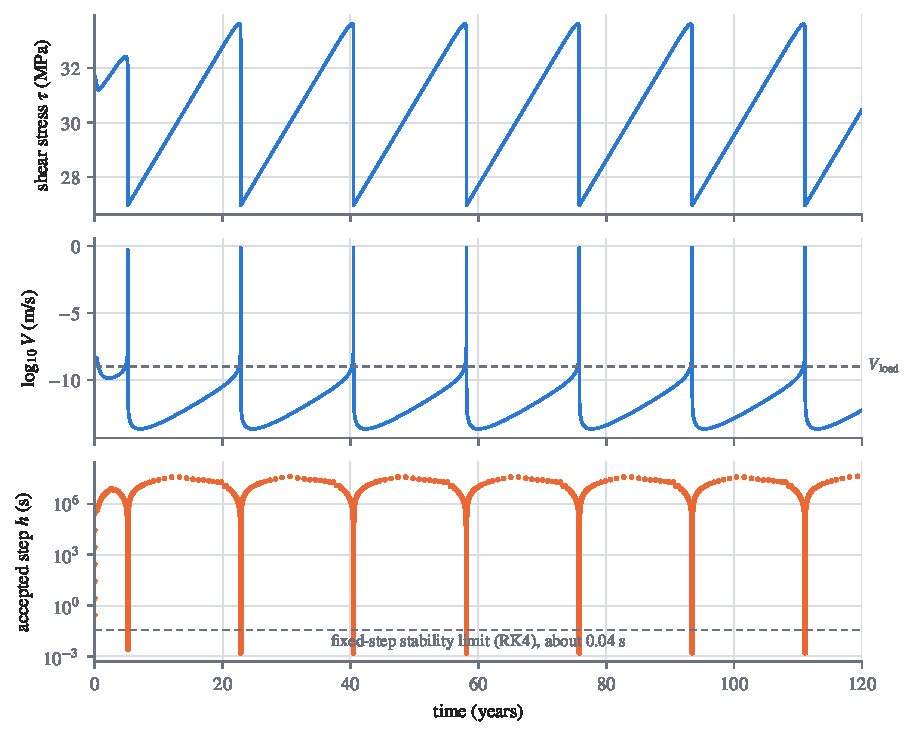
\includegraphics[width=0.88\textwidth]{slider_cycle}
\caption{Spring-block slider with $k=0.5\,k_{cr}$, integrated as the ODE system, Eq.~\eqref{eq:l3-ode}, with adaptive RK45 (relative tolerance $10^{-8}$). Top: shear stress; middle: slip rate on a logarithmic scale; bottom: size of every accepted time step (3\,782 steps in 120 yr). The step ranges from 1.7~ms during an event to 1.4~yr between events. The dashed line is a rough estimate of the largest stable step for a fixed-step RK4 scheme.}
\label{fig:l3-cycle}
\end{figure}

\subsection{Time integration: what the problem demands}

\paragraph{Time scales span ten orders of magnitude.} During an event the state variable relaxes at the rate $V/\Dc\sim80$~s$^{-1}$; between events the rate is $\Vl/\Dc=10^{-7}$~s$^{-1}$. A fixed time step must be small enough for the event and then be used for the 17.7 years in between. Using the stability bound of RK4 on the fastest rate gives $h\lesssim2.78/80\approx0.04$~s, so a fixed-step integration of one cycle would take about $1.5\times10^{10}$ steps. The adaptive integrator needs 538 steps per cycle: it takes steps of milliseconds during the event and steps of years in between (Figure~\ref{fig:l3-cycle}, bottom). This cost ratio is the argument for adaptive stepping.

\paragraph{The error tolerance controls accuracy, not stability.} Inside an event the smallest accepted step (1.7~ms) is about twenty times smaller than the stability limit just estimated. The step is therefore chosen by the accuracy requirement, and the problem is hard because it is rapidly varying, not because explicit integration is unstable. Whether to switch to an implicit method is decided by comparing these two limits; here no switch is needed.

\paragraph{Tolerance study.} Tightening the relative tolerance from $10^{-6}$ to $10^{-8}$ to $10^{-10}$ increases the number of steps in 120 yr from 1\,653 to 3\,782 to 9\,334, and changes the recurrence interval by less than $10^{-4}$~yr (17.65537, 17.65531, 17.65531). Cost grows slowly with accuracy, and a result that does not change under such a change in tolerance is converged in the sense that matters.

\subsection{Consistency checks}

\begin{enumerate}[itemsep=1pt,topsep=2pt]
\item \textbf{The first cycle is not representative.} In the reference run the first event slips 0.44~m and every later event slips 0.56~m, because the initial condition lies off the limit cycle. Results apply only once the solution is periodic: stress extrema, peak velocity and recurrence repeat to several digits.
\item \textbf{Slip balance.} Over a full cycle the spring stress returns to its starting value, so $\int\dot\tau\,\dd t=0$ and the slip per cycle equals $\Vl T_{rec}$. Here $10^{-9}\times17.655\times3.156\times10^{7}=0.557$~m, matching the integrated slip.
\item \textbf{Stress drop.} The drop in $\tau$ during an event must equal $k$ times the event slip. The computed drop is $33.62-26.96=6.67$~MPa; the slip it implies is $6.67/12.5=0.53$~m, close to the 0.56~m total (the small difference is the loading during the event).
\item \textbf{Peak velocity.} Radiation damping caps $V$ near (stress drop)/$\eta=6.67/5\approx1.3$~m/s. The computed peak, 0.77~m/s, is consistent in order of magnitude. A peak of $10^{3}$~m/s or $10^{-3}$~m/s would indicate an error in units or in $\eta$.
\item \textbf{Stiffness test.} The solution must change character at $k_{cr}$ (Table~\ref{tab:l3-kcr}). This is the cheapest test that the friction law, the aging law and the differentiated constraint have the correct signs.
\item \textbf{Constraint residual.} With $\tau$ carried as an extra state, $\tau-\tau_f-\eta V$ must stay at the integration tolerance (a few pascals at $10^{-8}$). A residual that is constant and non-zero from $t=0$ indicates an inconsistent initial condition; a residual that grows indicates a tolerance that is too loose.
\item \textbf{Tolerance test.} Repeating the run with the tolerance reduced by $10^2$ should leave event times and peak velocity unchanged in the reported digits.
\end{enumerate}

%======================================================================
\section{Frictional Heating and Heat Diffusion Away from the Fault}
\label{sec:l3-heat}
%======================================================================

\subsection{Heat source and governing equation}

The rate at which friction produces heat per unit fault area is
\begin{equation}
q(t)=\tau(t)\,V(t)\qquad[\text{W/m}^2].
\label{eq:l3-heat-rate}
\end{equation}
This is the quantity that connects Section~\ref{sec:l3-slider} to the present one: the slider provides $\tau(t)$ and $V(t)$, and the rock on either side of the fault must absorb $q$. In the limit of an infinitely thin slipping zone the heat is released at the plane $y=0$, where $y$ is the distance perpendicular to the fault, and spreads symmetrically, so each side receives $q_0=q/2$. Away from the fault the temperature rise $T(y,t)$ satisfies the diffusion equation
\begin{equation}
\frac{\partial T}{\partial t}=\alpha\,\frac{\partial^2T}{\partial y^2},\qquad y>0,
\label{eq:l3-diffusion}
\end{equation}
where $\alpha=k_{th}/(\rho c)$ is the thermal diffusivity, $k_{th}$ the thermal conductivity and $\rho c$ the volumetric heat capacity. We use $\alpha=10^{-6}$~m$^2$/s, $k_{th}=2.7$~W/(m\,K) and $\rho c=2.7\times10^6$~J/(m$^3$K) throughout. The fault enters the problem only through the boundary condition (Fourier's law),
\begin{equation}
-k_{th}\,\frac{\partial T}{\partial y}\Big|_{y=0}=q_0(t),\qquad T\to0\ \text{as } y\to\infty,
\label{eq:l3-bc}
\end{equation}
that is, a prescribed flux at $y=0$ and a fixed temperature far away. The pairing of a Neumann (flux) condition at the active boundary and a Dirichlet (value) condition at the inert one is typical of geophysical diffusion problems.

\begin{remark}[The same equation governs pore pressure]
Pore pressure $p(y,t)$ obeys $\partial p/\partial t=\alpha_{hy}\,\partial^2p/\partial y^2$ with a hydraulic diffusivity $\alpha_{hy}$, plus a coupling term in which rising temperature raises pressure. In a later lecture, pressure reduces the effective normal stress $\sigma$ in Eq.~\eqref{eq:l3-rsf}, which feeds back on $\tau$ and hence on $q$. A single tested diffusion solver will be used for both fields.
\end{remark}

\subsection{Scales before any grid is chosen}

The only length that the diffusion equation contains is the diffusion length $\delta(t)=\sqrt{\alpha t}$, the distance heat has spread by time $t$. With $\alpha=10^{-6}$~m$^2$/s:
\begin{center}
\small
\begin{tabular}{lcccc}
\toprule
elapsed time $t$ & 1 ms & 1 s & 12 s (one event) & 17.7 yr (one cycle) \\
\midrule
$\sqrt{\alpha t}$ & 30~$\mu$m & 1~mm & 3.5~mm & 24~m \\
\bottomrule
\end{tabular}
\end{center}
Two consequences shape every numerical decision later. First, the heated layer during an earthquake is millimetres thick, so the grid must resolve millimetres, not metres. Second, $\delta$ starts at zero and grows with time, so a grid fine enough at $t=1$~s may be too coarse at $t=1$~ms (Section~\ref{sec:l3-fd-verify}). Over the interseismic interval the heat spreads to tens of metres, a range of nearly four orders of magnitude in length scale; only the event and its aftermath are modeled here.

\subsection{How much heat, and how hot?}

Integrating $\tau V$ over one simulated event (the interval with $V>1$~mm/s, duration 12~s, slip 0.43~m, mean stress 29.7~MPa) gives a total of $Q=1.3\times10^{7}$~J/m$^2$, and the peak heating rate is $q_{max}=2.4\times10^{7}$~W/m$^2$.

A hand estimate of the temperature precedes any computation. For a constant flux $q_0$ switched on at $t=0$, the half-space solution is known in closed form,
\begin{equation}
T(y,t)=\frac{q_0}{k_{th}}\left[2\sqrt{\frac{\alpha t}{\pi}}\;e^{-y^2/4\alpha t}-y\,\mathrm{erfc}\!\left(\frac{y}{2\sqrt{\alpha t}}\right)\right],\qquad T(0,t)=\frac{2q_0}{k_{th}}\sqrt{\frac{\alpha t}{\pi}}.
\label{eq:l3-exact}
\end{equation}
Spread the event's heat uniformly over its duration: $q_0=Q/(2\times12\ \text{s})=5.3\times10^5$~W/m$^2$, so
\[
T(0,12\ \text{s})\approx\frac{2(5.3\times10^5)}{2.7}\sqrt{\frac{10^{-6}\times12}{\pi}}\approx 8\times10^{2}\ \text{K}.
\]
The full calculation with the actual $q(t)$, using the superposition integral for a time-varying flux,
\begin{equation}
T(0,t)=\frac{1}{k_{th}}\sqrt{\frac{\alpha}{\pi}}\int_0^t q_0(t')\,(t-t')^{-1/2}\,\dd t',
\end{equation}
gives a peak of about $2.3\times10^3$~K, reached about 10~s after the onset. The hand estimate is low by a factor of three because the heat is released mostly near the end of the event, and late heat has had less time to diffuse away. The sign of this bias is predictable, which makes the estimate a useful check.

Either number is unphysically large: it is above the melting temperature of rock. The reason is the assumption of a vanishing shear-zone thickness; real shear zones have finite width, and in the full model the fluid pressurization lowers $\tau$ as the fault heats, which reduces $q$. This feedback is exactly what the coupled model of later lectures will capture, and it is why temperature is a quantity that must be computed accurately and not guessed.

\begin{figure}[ht]
\centering
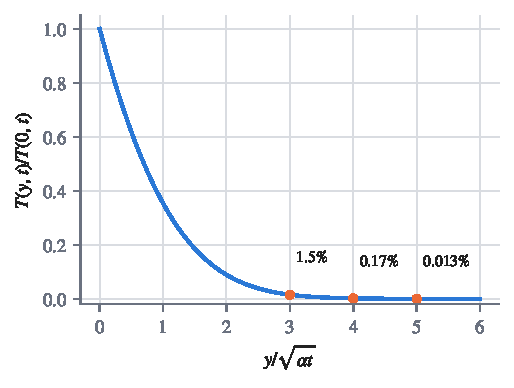
\includegraphics[width=0.52\textwidth]{heat_profile}
\caption{The constant-flux solution, Eq.~\eqref{eq:l3-exact}, normalized by its value at the fault, as a function of $y/\sqrt{\alpha t}$. The curve is universal: it has the same shape at all times, with only the length scale $\sqrt{\alpha t}$ changing. The temperature at $3\sqrt{\alpha t}$ is 1.5\% of the value at the fault, at $4\sqrt{\alpha t}$ it is 0.17\%, and at $5\sqrt{\alpha t}$ it is 0.013\%.}
\label{fig:l3-heat-profile}
\end{figure}

\subsection{The numerical problem}

The required quantity is $T(y,t)$, driven by a flux $q_0(t)$ that varies over many orders of magnitude and is itself produced by the slider. Discretizing only $y$ and keeping $t$ continuous turns Eq.~\eqref{eq:l3-diffusion} into a large system of ODEs, one per grid point, of the type treated in Section~\ref{sec:l3-slider} for two unknowns. This view (the method of lines) is used twice below: it explains the stability limit, and it determines how the diffusion solver is coupled to the slider.

%======================================================================
\section{Finite Differences for the Diffusion Equation}
\label{sec:l3-fd}
%======================================================================

\subsection{Structure of the analysis}

A finite-difference calculation is assessed by four questions, each with a failure mode that produces no error message.

\begin{enumerate}[itemsep=1pt,topsep=2pt]
\item \textbf{Is the discrete equation an approximation to the right equation, and of what order?} This is settled by a Taylor expansion (Sections~\ref{sec:l3-fd-space} and \ref{sec:l3-fd-time}).
\item \textbf{Is it stable?} An approximation can be accurate at every step and still blow up. A single dimensionless number decides (Section~\ref{sec:l3-fd-stab}).
\item \textbf{Are the boundary conditions as accurate as the interior, and do they conserve what should be conserved?} Boundaries are where order and energy are lost, and the loss is invisible on a plot (Section~\ref{sec:l3-fd-bc}).
\item \textbf{Is the complete implementation correct?} The tests are comparison with an exact solution, the rate at which the error falls under refinement, and a conserved quantity (Section~\ref{sec:l3-fd-verify}).
\end{enumerate}

For each of the four, the sections below give the criterion for a pass and the signature of a failure.

\subsection{Approximating derivatives on a grid}
\label{sec:l3-fd-space}

\begin{figure}[ht]
\centering
\begin{tikzpicture}[>=Stealth]
\def\dy{1.2}   % grid spacing in cm; nodes y_j = j*\dy, j = 0..9
% rock (y>0), mirror half-space (y<0), fault, far boundary
\fill[blue!6] (0,0) rectangle (10.8,2.4);
\draw[gray,dashed] (-1.8,0) rectangle (0,2.4);
\node[gray,font=\scriptsize,align=center] at (-0.9,1.2) {mirror image\\(no separate\\unknowns)};
\draw[orange!85!black,line width=2pt] (0,-0.05) -- (0,2.45);
\node[orange!85!black,font=\small,anchor=south] at (0,2.5) {fault, $y=0$};
\draw[line width=1.2pt] (10.8,0) -- (10.8,2.4);
\node[font=\small,anchor=west,align=left] at (10.95,1.2) {far boundary\\$T=0$};
% heat flux into the half-space
\draw[->,thick,orange!85!black] (0.05,0.3) -- (0.8,0.3);
\draw[->,thick,orange!85!black] (0.05,0.7) -- (0.8,0.7);
\node[orange!85!black,font=\scriptsize,anchor=west] at (0.08,1.0) {$q_0=q/2$};
% temperature profile (constant-flux solution) and its values at the nodes
\draw[thick,blue!70!black] plot[smooth] coordinates {(0.00,2.00) (0.60,1.55) (1.20,1.17) (1.80,0.86) (2.40,0.62) (3.00,0.43) (3.60,0.29) (4.20,0.19) (4.80,0.12) (5.40,0.08) (6.00,0.05) (6.60,0.03) (7.20,0.02) (7.80,0.01) (8.40,0.00) (9.00,0.00) (9.60,0.00) (10.20,0.00) (10.80,0.00)};
\foreach \j/\h in {0/2.00, 1/1.17, 2/0.62, 3/0.29, 4/0.12, 5/0.05, 6/0.02, 7/0.00, 8/0.00, 9/0.00} {
  \draw[gray,dotted] (\j*\dy,0) -- (\j*\dy,\h);
  \fill[blue!70!black] (\j*\dy,\h) circle (1.6pt);
  \fill (\j*\dy,0) circle (2pt);
}
\node[blue!70!black,font=\scriptsize,anchor=south west] at (4.85,0.12) {$T_j^n$};
% node axis and labels
\draw[->] (-1.8,0) -- (13.2,0) node[right,font=\small] {$y$};
\draw[fill=white] (-1.2,0) circle (2pt);
\node[gray,font=\scriptsize,anchor=north] at (-1.2,-0.62) {ghost node};
\foreach \x/\l in {-1.2/y_{-1}, 0/y_0, 1.2/y_1, 2.4/y_2, 3.6/\cdots, 4.8/y_{j-1},
                   6/y_j, 7.2/y_{j+1}, 8.4/\cdots, 9.6/\cdots, 10.8/y_N}
  \node[below,font=\small] at (\x,-0.08) {$\l$};
\draw[decorate,decoration={brace,amplitude=3pt,mirror}] (0,-0.95) -- (1.2,-0.95)
  node[midway,below=3pt,font=\scriptsize] {$\Delta y$};
\draw[decorate,decoration={brace,amplitude=3pt,mirror}] (6,-0.95) -- (7.2,-0.95)
  node[midway,below=3pt,font=\scriptsize] {$\Delta y$};
% diffusion length and domain size
\draw[<->] (0,2.95) -- (2.16,2.95) node[midway,above,font=\scriptsize] {$\sqrt{\alpha t}$};
\draw[<->] (0,3.65) -- (10.8,3.65)
  node[midway,above,font=\scriptsize] {$y_N\gtrsim5\sqrt{\alpha\,t_{final}}$};
\draw[dotted,gray] (2.16,2.4) -- (2.16,3.0);
\draw[dotted,gray] (10.8,2.4) -- (10.8,3.7);
\end{tikzpicture}
\caption{Spatial discretization next to the fault. Frictional heat generated on the plane $y=0$ enters the half-space $y\ge0$ at $q_0=q/2$ per side. The temperature $T_j^n$ is stored at the nodes $y_j=j\,\Delta y$, $j=0,\dots,N$, and $T=0$ is imposed at the far boundary $y_N$. The node $y_{-1}$ is a fictitious ghost value used for the flux condition (Section~\ref{sec:l3-fd-bc}). The heated layer has a thickness of order $\sqrt{\alpha t}$, so $y_N$ must exceed several multiples of $\sqrt{\alpha t_{final}}$. The profile shown is the constant-flux solution, Eq.~\eqref{eq:l3-exact}.}
\label{fig:l3-grid}
\end{figure}

Replace the half-line $y\ge0$ by points $y_j=j\,\Delta y$, $j=0,\dots,N$, with $y_0=0$ at the fault and $y_N$ the far boundary. Let $T_j^n\approx T(y_j,t^n)$ with $t^n=n\,\Delta t$. To approximate $\partial^2T/\partial y^2$ at an interior point, expand the neighbors in Taylor series about $y_j$ at fixed time:
\begin{align}
T_{j+1}&=T_j+\Delta y\,T_j'+\tfrac12\Delta y^2T_j''+\tfrac16\Delta y^3T_j'''+\tfrac1{24}\Delta y^4T_j''''+\order{\Delta y^5},\\
T_{j-1}&=T_j-\Delta y\,T_j'+\tfrac12\Delta y^2T_j''-\tfrac16\Delta y^3T_j'''+\tfrac1{24}\Delta y^4T_j''''+\order{\Delta y^5}.
\end{align}
where primes denote $\partial/\partial y$ evaluated at $y_j$, at fixed time (the time index is suppressed in this calculation).

Adding the two, the odd-order terms cancel exactly:
\begin{equation}
\frac{\partial^2T}{\partial y^2}\Big|_{y_j}=\frac{T_{j+1}-2T_j+T_{j-1}}{\Delta y^2}-\frac{\Delta y^2}{12}\,T_j''''+\order{\Delta y^4}.
\label{eq:l3-central}
\end{equation}
The first term on the right is the \textbf{central difference}. The leading truncation error is proportional to $\Delta y^2$: the scheme is second order in space, and its error is largest where the solution has sharp fine-scale structure ($T''''$ large), such as the first few $\sqrt{\alpha t}$ at early times.

The cancellation depends on $y_j$ sitting exactly midway between its neighbors. A first derivative from a one-sided difference does not enjoy it:
\begin{equation}
\frac{\partial T}{\partial y}\Big|_{y_j}=\frac{T_{j+1}-T_j}{\Delta y}+\order{\Delta y},\qquad
\frac{\partial T}{\partial y}\Big|_{y_j}=\frac{T_{j+1}-T_{j-1}}{2\Delta y}+\order{\Delta y^2}.
\label{eq:l3-first}
\end{equation}
The one-sided formula is first order and the centered one is second order, at the same cost. This matters at the fault, where one neighbor is missing (Section~\ref{sec:l3-fd-bc}).

\subsection{Marching in time: the explicit scheme}
\label{sec:l3-fd-time}

The explicit scheme applies forward Euler in time, as in the earlier ODE lectures, at each grid point, together with the central difference in space. Write the diffusion equation, Eq.~\eqref{eq:l3-diffusion}, at the node $(y_j,t^n)$:
\begin{equation}
\frac{\partial T}{\partial t}\bigg|_j^n=\alpha\,\frac{\partial^2T}{\partial y^2}\bigg|_j^n.
\end{equation}
For the time derivative, expand $T$ forward in time about $t^n$ at fixed $y_j$:
\begin{equation}
T_j^{n+1}=T_j^n+\Delta t\,\frac{\partial T}{\partial t}\bigg|_j^n+\frac{\Delta t^2}{2}\frac{\partial^2T}{\partial t^2}\bigg|_j^n+\order{\Delta t^3},
\end{equation}
which gives
\begin{equation}
\frac{\partial T}{\partial t}\bigg|_j^n=\frac{T_j^{n+1}-T_j^n}{\Delta t}-\frac{\Delta t}{2}\frac{\partial^2T}{\partial t^2}\bigg|_j^n+\order{\Delta t^2}.
\end{equation}
For the space derivative, use Eq.~\eqref{eq:l3-central} at time level $n$:
\begin{equation}
\frac{\partial^2T}{\partial y^2}\bigg|_j^n=\frac{T_{j+1}^n-2T_j^n+T_{j-1}^n}{\Delta y^2}-\frac{\Delta y^2}{12}\frac{\partial^4T}{\partial y^4}\bigg|_j^n+\order{\Delta y^4}.
\end{equation}
Substituting both into the diffusion equation and collecting the terms that contain higher derivatives on the right-hand side,
\begin{equation}
\frac{T_j^{n+1}-T_j^n}{\Delta t}=\alpha\,\frac{T_{j+1}^n-2T_j^n+T_{j-1}^n}{\Delta y^2}+\underbrace{\frac{\Delta t}{2}\frac{\partial^2T}{\partial t^2}-\alpha\frac{\Delta y^2}{12}\frac{\partial^4T}{\partial y^4}}_{\text{truncation error}\;=\;\order{\Delta t}+\order{\Delta y^2}}.
\end{equation}
The scheme is obtained by dropping the truncation error. The result contains a single unknown, $T_j^{n+1}$, because every other quantity is evaluated at time level $n$. Multiplying by $\Delta t$ and solving for $T_j^{n+1}$ gives the FTCS (forward-time, centered-space) update
\begin{equation}
T_j^{n+1}=T_j^n+s\,\big(T_{j+1}^n-2T_j^n+T_{j-1}^n\big),\qquad s\equiv\frac{\alpha\,\Delta t}{\Delta y^2},
\label{eq:l3-ftcs}
\end{equation}
where $s$ is the only combination of $\alpha$, $\Delta t$ and $\Delta y$ that enters the update.

The dimensionless \textbf{diffusion number} $s$ is the most important quantity in the scheme. Equation~\eqref{eq:l3-ftcs} can be rewritten as $T_j^{n+1}=(1-2s)T_j^n+sT_{j+1}^n+sT_{j-1}^n$, a weighted average with weights summing to one. For $s\le\tfrac12$ all weights are non-negative, so each new value lies between the smallest and largest of the three old values and the scheme cannot create new extrema, which is the correct behavior of diffusion. For $s>\tfrac12$ the middle weight is negative, and the average interpretation is lost.

\begin{figure}[ht]
\centering
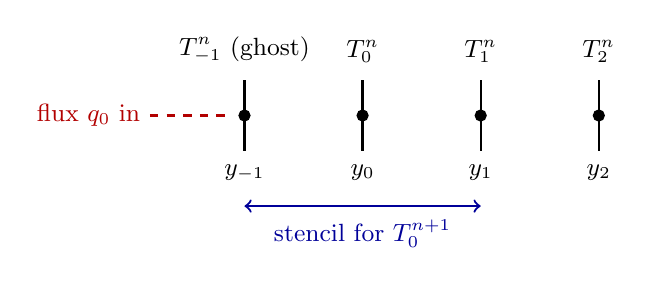
\begin{tikzpicture}[scale=1.0]
\def\dy{1.5}
\foreach \j/\lab in {-1/{-1}, 0/{0}, 1/{1}, 2/{2}} {
  \draw[thick] (\j*\dy,0) -- (\j*\dy,0.9);
  \filldraw[black] (\j*\dy,0.45) circle (2pt);
  \node[below] at (\j*\dy,-0.05) {\small $y_{\lab}$};
}
\node[above] at (-\dy,1.0) {\small $T_{-1}^n$ (ghost)};
\node[above] at (0,1.0) {\small $T_0^n$};
\node[above] at (\dy,1.0) {\small $T_1^n$};
\node[above] at (2*\dy,1.0) {\small $T_2^n$};
\draw[<->,thick,blue!60!black] (-\dy,-0.7) -- (\dy,-0.7);
\node[below,blue!60!black] at (0,-0.75) {\small stencil for $T_0^{n+1}$};
\draw[dashed,red!70!black,thick] (-1.8*\dy,0.45) -- (-\dy-0.15,0.45);
\node[left,red!70!black] at (-1.8*\dy,0.45) {\small flux $q_0$ in};
\end{tikzpicture}
\caption{The explicit stencil. The update at node $j$ uses the old values at $j-1$, $j$, $j+1$ and nothing from the new time level. At the fault ($j=0$) the node $j=-1$ does not exist physically, so a ghost value is constructed from the flux condition (Section~\ref{sec:l3-fd-bc}).}
\label{fig:l3-stencil}
\end{figure}

\subsection{Stability}
\label{sec:l3-fd-stab}

The truncation errors above are $\order{\Delta t}+\order{\Delta y^2}$, so FTCS is consistent. Consistency is not sufficient: forward Euler on $\dot y=\lambda y$ is consistent for every $h$ yet unstable unless $|1+h\lambda|\le1$, i.e.\ $h\le2/|\lambda|$ for real negative $\lambda$. The same applies here, and there are two independent ways to see what $s$ must satisfy.

\paragraph{Fourier (von Neumann) analysis.} Insert a single wave $T_j^n=\xi^n e^{\mathrm{i}\theta j}$, where $\theta=k\Delta y\in[-\pi,\pi]$ is the phase advance per cell, into Eq.~\eqref{eq:l3-ftcs}. The per-step amplification factor of the wave is
\begin{equation}
\xi(\theta)=1-4s\sin^2\!\frac{\theta}{2}\in[1-4s,\,1].
\label{eq:l3-vn}
\end{equation}
Stability needs $|\xi|\le1$ for every representable wave. The dangerous one is the checkerboard $\theta=\pi$ (alternating sign from node to node), for which $\xi=1-4s$; requiring $|1-4s|\le1$ gives
\begin{equation}
\boxed{\,s\le\tfrac12\quad\Longleftrightarrow\quad\Delta t\le\frac{\Delta y^2}{2\alpha}\,}.
\label{eq:l3-bound}
\end{equation}

\paragraph{Method of lines.} Discretizing only in space leaves the time derivative continuous. With $T_0=T_N=0$ imposed (homogeneous Dirichlet conditions, for this illustration) the interior values $T_1,\dots,T_{N-1}$ obey
\begin{equation}
\frac{\dd T_j}{\dd t}=\frac{\alpha}{\Delta y^2}\big(T_{j+1}-2T_j+T_{j-1}\big),\qquad j=1,\dots,N-1,
\end{equation}
which is a linear ODE system. Written out as a vector equation,
\begin{equation}
\frac{\dd}{\dd t}
\begin{pmatrix}T_1\\T_2\\T_3\\\vdots\\T_{N-2}\\T_{N-1}\end{pmatrix}
=\frac{\alpha}{\Delta y^2}
\begin{pmatrix}
-2 & 1 & & & & \\
1 & -2 & 1 & & & \\
 & 1 & -2 & 1 & & \\
 & & \ddots & \ddots & \ddots & \\
 & & & 1 & -2 & 1\\
 & & & & 1 & -2
\end{pmatrix}
\begin{pmatrix}T_1\\T_2\\T_3\\\vdots\\T_{N-2}\\T_{N-1}\end{pmatrix},
\qquad\text{i.e.}\qquad
\dot{\mathbf T}=\frac{\alpha}{\Delta y^2}\,D\,\mathbf T,
\end{equation}
where $D$ is the $(N-1)\times(N-1)$ tridiagonal matrix with $-2$ on the diagonal and $1$ on the two adjacent diagonals; empty entries are zero. The matrix $\alpha D/\Delta y^2$ plays the role of the Jacobian in the ODE lectures. Its eigenvalues are known in closed form,
\begin{equation}
\lambda_k=-\frac{4\alpha}{\Delta y^2}\sin^2\!\frac{k\pi}{2N},\qquad k=1,\dots,N-1,
\end{equation}
all real and negative. The most negative one tends to $\lambda_{max}\to-4\alpha/\Delta y^2$ as the grid is refined. Applying forward Euler to this system gives
\begin{equation}
\mathbf T^{n+1}=\mathbf T^n+\Delta t\,\frac{\alpha}{\Delta y^2}\,D\,\mathbf T^n=(I+s\,D)\,\mathbf T^n,
\end{equation}
which is Eq.~\eqref{eq:l3-ftcs} written for all nodes at once. The eigenvalues of $I+sD$ are $1+s\,\mu_k$, with $\mu_k=-4\sin^2(k\pi/2N)\in(-4,0)$, and forward Euler is stable if all of them lie in $[-1,1]$. The most restrictive is $k=N-1$, where $\mu_k\to-4$, so the condition is $|1-4s|\le1$, i.e.\ $\Delta t\le2/|\lambda_{max}|=\Delta y^2/(2\alpha)$. This is the same bound as above, obtained without Fourier analysis, and the agreement of the two derivations is itself a check on the algebra.

This means that refining the grid makes the ODE system stiffer, with a rate that grows as $1/\Delta y^2$. For $\alpha=10^{-6}$~m$^2$/s: $\Delta y=0.1$~mm requires $\Delta t\le5$~ms; $\Delta y=10$~$\mu$m requires $\Delta t\le50$~$\mu$s. Resolution is paid for twice, once in the number of nodes and once in the number of steps.

\begin{figure}[ht]
\centering
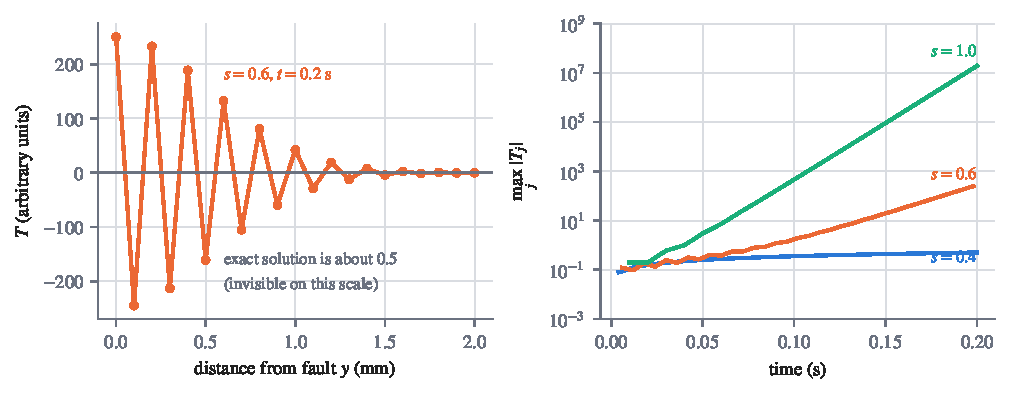
\includegraphics[width=0.96\textwidth]{fd_instability}
\caption{Violating $s\le1/2$ ($\Delta y=0.1$~mm, $\alpha=1$~mm$^2$/s, unit flux gradient). Left: profile near the fault at $t=0.2$~s for $s=0.6$; the solution alternates in sign from node to node with amplitude of order 250, whereas the exact value is about 0.5. Right: the largest absolute value of $T$ over the grid as a function of time; for $s=0.4$ it is stable and for $s=0.6$ and $s=1$ it grows geometrically.}
\label{fig:l3-instability}
\end{figure}

\paragraph{Appearance of the instability.} An unstable run does not stop with an error message; it produces a checkerboard whose amplitude grows by $|1-4s|$ at every step (Figure~\ref{fig:l3-instability}). A mild violation is more dangerous than a gross one, because it can look correct for a long time. With $\Delta y=0.1$~mm and $\alpha=1$~mm$^2$/s, the temperature at the fault for $s=0.51$ is $0.518$ at $t=0.2$~s against an exact $0.505$ (a 3\% error that could be taken for discretization error), then $-2.0$ at $t=1$~s, $-4.8\times10^3$ at $t=2$~s and $-1.6\times10^{10}$ at $t=4$~s. At $s=0.5$ the result remains accurate at all these times. The value of $s$ should therefore be checked explicitly; a variable time step is the usual way an $s$ slightly above one-half goes unnoticed.

\paragraph{Consistency plus stability gives convergence.} The Lax equivalence theorem states that, for a well-posed linear problem, a consistent and stable scheme converges as the grid is refined, and that a scheme which converges must be both. This is why checking the order of the truncation error and checking $s\le\frac12$ are the two halves of one guarantee, and why a convergence study (Section~\ref{sec:l3-fd-verify}) can be trusted only after stability has been established.

\subsection{Boundary conditions}
\label{sec:l3-fd-bc}

\paragraph{Far boundary.} At $y_N$ we impose $T=0$. This is correct only as long as no appreciable heat has reached it. The solution at $y=c\sqrt{\alpha t}$ relative to the fault value is 1.5\%, 0.17\% and 0.013\% for $c=3,4,5$ (Figure~\ref{fig:l3-heat-profile}), so a conservative rule is
\begin{equation}
y_N\gtrsim5\sqrt{\alpha\,t_{final}},
\label{eq:l3-domain}
\end{equation}
re-checked whenever the simulated time changes.

\paragraph{Fault boundary.} The condition $-k_{th}\,\partial_yT=q_0$ involves a derivative, and the update at $j=0$ needs $T_{-1}$, which does not exist. A \textbf{ghost point} is a fictitious value chosen so that the centered difference of Eq.~\eqref{eq:l3-first} at $j=0$ reproduces the boundary condition. The flux enters the rock, so the temperature decreases away from the fault, $\partial_yT|_0=-q_0/k_{th}$, and
\begin{equation}
\frac{T_1^n-T_{-1}^n}{2\Delta y}=-\frac{q_0}{k_{th}}\;\;\Longrightarrow\;\;T_{-1}^n=T_1^n+\frac{2\Delta y\,q_0}{k_{th}}.
\end{equation}
Substituting into Eq.~\eqref{eq:l3-ftcs} at $j=0$,
\begin{equation}
T_0^{n+1}=T_0^n+2s\,(T_1^n-T_0^n)+\frac{2s\,\Delta y\,q_0(t^n)}{k_{th}}.
\label{eq:l3-bc-update}
\end{equation}
There is a physical reading of the two factors of 2. Node 0 owns only the half-cell of width $\Delta y/2$ next to the boundary. Heat balance on it reads $(\Delta y/2)\,\dot T_0=\alpha(T_1-T_0)/\Delta y+\alpha q_0/k_{th}$, and multiplying by $\Delta t$ gives Eq.~\eqref{eq:l3-bc-update} exactly. This control-volume view is how the same condition is derived in the finite-volume method, and it shows what goes wrong if the factors are dropped.

\paragraph{Errors in the boundary treatment.} Each of the following gives a stable, smooth-looking solution at $\Delta y=0.1$~mm, $\alpha=1$~mm$^2$/s, $t=1$~s with unit flux gradient. The exact value is $T(0)=1.1284$ and the exact heat content $\int T\,\dd y=\alpha t\,q_0/k_{th}=1$.

\begin{center}
\small
\begin{tabular}{lccc}
\toprule
boundary treatment & $T(0)$ & heat content & error decays as \\
\midrule
ghost point, Eq.~\eqref{eq:l3-bc-update} & 1.1277 & 1.000 & $\Delta y^2$ \\
node treated as a full cell (factors 2 dropped) & 1.0791 & 0.946 & $\Delta y$ \\
one-sided gradient $T_0=T_1+\Delta y\,q_0/k_{th}$ & 1.1790 & 1.059 & $\Delta y$ \\
sign of the flux reversed & $-1.1277$ & $-1.000$ & (obvious) \\
\bottomrule
\end{tabular}
\end{center}
The reversed sign shows itself in the first plot. The other two errors are about 5\% and look like ordinary discretization error; they reveal themselves only through the convergence rate (the error falls by a factor of 2, not 4, when $\Delta y$ is halved) and through the heat balance (Figure~\ref{fig:l3-convergence}). A related mistake, forgetting that the flux splits into two sides ($q_0=q/2$), multiplies every temperature by exactly 2 and can be caught only by comparing the heat in the rock with $\tfrac12\int\tau V\,\dd t$.

\subsection{Preview: implicit time stepping}

The bound $\Delta t\le\Delta y^2/(2\alpha)$ is expensive when coupled to the slider. With $\Delta y=0.1$~mm, covering a single 17.7~yr interseismic interval with 5~ms steps takes about $10^{11}$ steps, although the slider itself needs only a few hundred. Evaluating the spatial difference at the new time level,
\begin{equation}
\frac{T_j^{n+1}-T_j^n}{\Delta t}=\alpha\,\frac{T_{j+1}^{n+1}-2T_j^{n+1}+T_{j-1}^{n+1}}{\Delta y^2},
\end{equation}
gives BTCS, with $\xi(\theta)=1/\big(1+4s\sin^2(\theta/2)\big)\in(0,1]$ for every $s>0$ and thus no stability limit on $\Delta t$. The price is a tridiagonal linear system at each step, which is cheap. This is the backward Euler method from the ODE lectures applied to the stiff system above. The coupled calculation in a later lecture will make this switch, and the stability analysis here is the justification for it.

\subsection{Verification}
\label{sec:l3-fd-verify}

Visual plausibility of a profile is not a test. Four checks are used, each with a numerical outcome. The benchmark throughout is Eq.~\eqref{eq:l3-exact}, computed in units of mm and seconds with $\alpha=1$~mm$^2$/s and $q_0/k_{th}=1$~K/mm, so $T(0,t)=2\sqrt{t/\pi}$ and $T(0,1\ \text{s})=1.1284$~K.

\paragraph{1. Compare with the exact solution.} Equation~\eqref{eq:l3-exact} is the only closed-form solution needed. An implementation that does not reproduce it for a constant flux cannot be relied on for a variable flux.

\paragraph{2. Refine and read the rate.} Reduce $\Delta y$ by 2 at a time step small enough that time error is negligible; the error in $T(0)$ at $t=1$~s should fall by a factor of 4.

\begin{center}
\small
\begin{tabular}{lcccc}
\toprule
$\Delta y$ (mm) & 0.4 & 0.2 & 0.1 & 0.05 \\
\midrule
error in $T(0)$ & $1.15\times10^{-2}$ & $2.83\times10^{-3}$ & $7.04\times10^{-4}$ & $1.75\times10^{-4}$ \\
ratio to previous & --- & 4.05 & 4.02 & 4.03 \\
\bottomrule
\end{tabular}
\end{center}
In time, at fixed $\Delta y=0.1$~mm, halving $\Delta t$ halves the error (ratios 2.01, 2.01, 2.02, forward Euler is first order). If $s$ is kept fixed at 0.25, then $\Delta t\propto\Delta y^2$ and the combined error falls by a factor of 4.00 per halving of $\Delta y$. The scheme behaves as second order in $\Delta y$ along any path of constant $s$, which is how it is used in practice. An error that falls by a factor of 2 where 4 is expected indicates that a boundary or another lower-order component limits the accuracy (Figure~\ref{fig:l3-convergence}).

\begin{figure}[ht]
\centering
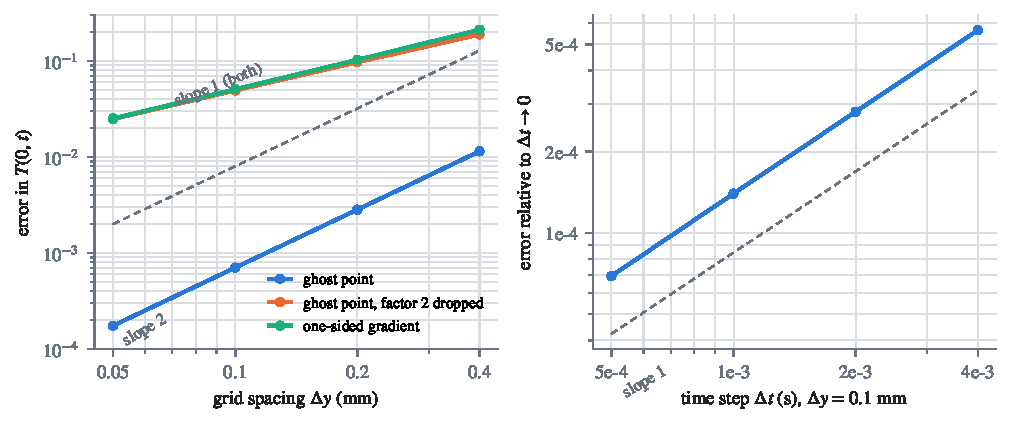
\includegraphics[width=0.96\textwidth]{fd_convergence}
\caption{Left: error in the fault temperature at $t=1$~s against grid spacing for the ghost-point boundary and for the two lower-order treatments of the previous table. Right: error against time step at $\Delta y=0.1$~mm, relative to the limit $\Delta t\to0$. The ghost-point treatment follows a slope of 2; the other two have slope 1 and lose a factor of about 70 in accuracy at $\Delta y=0.1$~mm.}
\label{fig:l3-convergence}
\end{figure}

\paragraph{3. Check a conserved quantity.} The heat content $\int T\,\dd y$ must equal $\alpha\,t\,q_0/k_{th}$, independent of the detailed profile. It is a one-line check, it catches errors in the boundary, and the table above shows it reading 0.946 and 1.059 for the two faulty closures. Two cautions. The integral must be evaluated with the trapezoid rule (half weight at the boundary node), because the correct scheme itself gives 1.056 with a plain sum; the checking tool can be wrong too. And when the calculation is coupled to the slider, the heat in the rock must equal $\tfrac12\int\tau V\,\dd t$.

\paragraph{4. Check the domain and the early times.} For a unit flux, with $\Delta y=0.1$~mm, $\Delta t=10^{-3}$~s, the error in $T(0)$ is $5\times10^{-5}$ times the exact value when the domain is $3.2\sqrt{\alpha t}$ long ($t=10$~s, $L=10$~mm), 2.2\% for $1.6\sqrt{\alpha t}$ and 20\% for $0.9\sqrt{\alpha t}$. A domain that is too short does not generate any artefact visible in the interior; it simply lowers the temperature through the Dirichlet condition. The grid can also be too coarse for early times: for $\Delta y=0.1$~mm the relative error in $T(0)$ is 49\% at $t=1$~ms ($\sqrt{\alpha t}/\Delta y=0.3$), 7.2\% at 10~ms (1.0), 0.62\% at 0.1~s (3.2) and 0.061\% at 1~s (10). A good working rule is $\sqrt{\alpha t}\gtrsim3\,\Delta y$; at earlier times the numerical solution is only qualitatively right. The same grid can therefore pass a refinement test at 1~s and fail one at 1~ms.

\subsection{Symptoms and likely causes}

\begin{center}
\small
\renewcommand{\arraystretch}{1.15}
\begin{tabular}{p{0.38\textwidth}p{0.55\textwidth}}
\toprule
Symptom & Likely cause \\
\midrule
Alternating signs between nodes, amplitude growing & $s>\tfrac12$, Eq.~\eqref{eq:l3-bound}; print $s$ at each step \\
Temperature negative where heat is being injected & sign of the flux in the ghost-point update \\
Smooth profile but error halves (not quarters) under refinement & boundary closure of low order; node treated as a full cell \\
Heat content differs from $\alpha t q_0/k_{th}$ by a few percent & boundary update; trapezoid weights in the check \\
Temperature exactly twice the expected value & flux not divided between the two sides \\
Temperature at the fault drops when the domain is shortened & domain shorter than $5\sqrt{\alpha t_{final}}$ \\
Early-time error large, late-time error small & grid coarse compared with $\sqrt{\alpha t}$ at early $t$ \\
Slider: first events differ from later ones & spin-up transient; discard until periodic \\
Slider: velocity cap far from (stress drop)/$\eta$ & units, $\eta$, or the term $\eta V$ missing from the denominator of Eq.~\eqref{eq:l3-ode} \\
Slider: cycles correct but $\tau$ offset by a constant & initial condition violating the constraint, Eq.~\eqref{eq:l3-constraint} \\
\bottomrule
\end{tabular}
\end{center}

%======================================================================
\section{Summary}
\label{sec:l3-summary}
%======================================================================

\begin{itemize}[itemsep=2pt,topsep=2pt]
\item The spring-block slider is two ODEs plus one algebraic constraint. Differentiating the constraint gives an ODE system in $(\ln V,\theta)$, which an adaptive Runge--Kutta method integrates with steps from milliseconds to years in one run. The initial condition must satisfy the constraint, and the constraint residual should be monitored. Check the slip balance, the stress drop, the peak velocity and the transition at $k_{cr}$.
\item Frictional heating $q=\tau V$ drives a diffusion problem with a flux boundary condition at the fault. The diffusion length $\sqrt{\alpha t}$ sets the grid, the domain and a hand estimate of the temperature, and the constant-flux solution is the benchmark.
\item The explicit finite-difference scheme is second order in space and first order in time. It is stable only if $s=\alpha\Delta t/\Delta y^2\le\tfrac12$, which can be derived in two ways that agree. The cost grows as $1/\Delta y^2$.
\item Boundary conditions are where silent errors enter. The ghost-point treatment is second order and conserves heat; two plausible alternatives are first order and look correct.
\item Verification means a benchmark, the observed convergence rate, a conservation check, and checks of the domain size and the early-time resolution.
\end{itemize}

%======================================================================
\section{Notation}
\label{sec:l3-notation}
%======================================================================

\begin{center}
\small
\begin{tabular}{ll}
\toprule
Symbol & Meaning \\
\midrule
$\tau$, $\tau_f$ & shear stress; frictional strength \\
$V$, $\Vl$ & slip rate; plate (loading) velocity \\
$\theta$, $\Dc$ & state variable; characteristic slip distance \\
$\sigma$ & effective normal stress \\
$a$, $b$, $\mu^*$, $V^*$ & rate-and-state parameters and reference values \\
$k$, $k_{cr}$ & spring stiffness; critical stiffness \\
$\eta=G/(2\beta)$ & radiation-damping coefficient \\
$x=\ln(V/V^*)$ & state variable replacing $V$ \\
$q=\tau V$, $q_0=q/2$ & frictional heating rate; flux into one side \\
$T(y,t)$ & temperature rise; $y$ is distance from the fault \\
$\alpha$, $k_{th}$, $\rho c$ & thermal diffusivity, conductivity, heat capacity \\
$\sqrt{\alpha t}$ & diffusion length \\
$\Delta y$, $\Delta t$, $T_j^n$ & grid spacing, time step, grid value \\
$s=\alpha\Delta t/\Delta y^2$ & diffusion number \\
$\xi(\theta)$ & amplification factor of a Fourier mode \\
\bottomrule
\end{tabular}
\end{center}

%======================================================================
\section{Suggested Reading}
\label{sec:l3-reading}
%======================================================================

\begin{itemize}[itemsep=2pt,topsep=2pt]
\item J.\,R.\ Rice and A.\,L.\ Ruina (1983), Stability of steady frictional slipping, \emph{J.\ Appl.\ Mech.}\ 50, 343--349. The linear stability analysis behind Eq.~\eqref{eq:l3-kcr}.
\item J.\,R.\ Rice (1993), Spatio-temporal complexity of slip on a fault, \emph{J.\ Geophys.\ Res.}\ 98, 9885--9907. The radiation-damping approximation and the aging-law slider.
\item H.\,S.\ Carslaw and J.\,C.\ Jaeger (1959), \emph{Conduction of Heat in Solids}, 2nd ed., Oxford University Press. The solution Eq.~\eqref{eq:l3-exact} and its relatives.
\item R.\,J.\ LeVeque (2007), \emph{Finite Difference Methods for Ordinary and Partial Differential Equations}, SIAM. Chapters on the heat equation, stability and boundary conditions.
\item J.\,R.\ Rice (2006), Heating and weakening of faults during earthquake slip, \emph{J.\ Geophys.\ Res.}\ 111, B05311. Where the temperature estimate of Section~\ref{sec:l3-heat} leads.
\end{itemize}

%======================================================================
\section{Practice Problems: Numerical Pitfalls}
\label{sec:l3-problems}
%======================================================================

\subsection*{Problem 1: initial transient in the slider}

Integration of the slider of Section~\ref{sec:l3-slider} gives a slip of 0.44~m in the first event and 0.56~m in all later events, with a recurrence interval of 17.655~yr. Determine whether this indicates an error.

\solution It does not. The initial condition ($\theta$ at half its steady-state value) lies off the limit cycle, and the first event occurs at 5.2~yr, before a full recurrence interval has elapsed, so the first cycle is a transient. The slip balance holds for the later events: $\Vl T_{rec}=10^{-9}\times17.655\times3.156\times10^7=0.557$~m. An actual error would appear as later events that differ from $\Vl T_{rec}$ or from one another.

\subsection*{Problem 2: the cost of a fixed step}

Estimate the number of steps a fixed-step RK4 integration needs for one cycle, using the largest slip rate $V_{max}=0.77$~m/s, $\Dc=10$~mm and the RK4 real-axis stability limit $|h\lambda|\le2.78$. Compare with the 538 steps taken by the adaptive integrator.

\solution The fastest rate is $\lambda\approx V_{max}/\Dc=77$~s$^{-1}$, so $h\le2.78/77=0.036$~s. One cycle is $5.57\times10^{8}$~s, giving $1.5\times10^{10}$ steps. The adaptive integrator takes $3\times10^{7}$ times fewer steps. The estimate is a lower bound on the fixed-step cost, since accuracy may require smaller steps than stability. The cost is set by the ratio of the fastest to the slowest time scale, which an adaptive integrator does not pay.

\subsection*{Problem 3: a time step that is slightly too large}

For $\Delta y=0.1$~mm and $\alpha=1$~mm$^2$/s, the explicit scheme is run with $\Delta t=5.1$~ms. At $t=0.2$~s the fault temperature is $0.518$, against an exact $0.505$, a 3\% error. Determine whether this error is a discretization error.

\solution It is not. Here $s=0.51>\tfrac12$. The checkerboard mode grows by $|1-4s|=1.04$ per step, which is not yet visible at 0.2~s (40 steps) but which has taken the fault temperature to $-2.0$ at $t=1$~s, $-4.8\times10^3$ at 2~s and $-1.6\times10^{10}$ at 4~s. At $s=0.5$ the same code is accurate at all four times. The 3\% error was the beginning of the instability, not a discretization error. The stable choice is $\Delta t\le\Delta y^2/(2\alpha)=5$~ms.

\subsection*{Problem 4: two boundary errors that look like accuracy limits}

At $\Delta y=0.1$~mm, one code gives $T(0)=1.079$ and heat content 0.946 at $t=1$~s; another gives $T(0)=1.179$ and heat content 1.059. The exact values are 1.128 and 1.000. Halving $\Delta y$ in each code gives $T(0)=1.104$ and $T(0)=1.154$ respectively. Identify the error in each and explain why neither is visible in a plot of the profile.

\solution Halving $\Delta y$ reduces the error from $4.9\times10^{-2}$ to $2.5\times10^{-2}$ in the first code and from $5.1\times10^{-2}$ to $2.5\times10^{-2}$ in the second: factors of 2, instead of the 4 that a second-order scheme gives. Both have a first-order boundary. In the first code the factors of 2 in Eq.~\eqref{eq:l3-bc-update} were dropped, so the boundary node is treated as a full cell and it holds too little heat (0.946). In the second the gradient was imposed with a one-sided difference, $T_0=T_1+\Delta y\,q_0/k_{th}$, which has an $\order{\Delta y}$ error and gives too much heat (1.059). Both profiles are smooth and about 5\% off, so a plot will not reveal either; the convergence rate and the heat content do.

\subsection*{Problem 5: domain and early times}

A simulation to $t_{final}=10$~s with $\alpha=1$~mm$^2$/s uses a domain of length $L=3$~mm and $\Delta y=0.1$~mm, and is repeated to $t=1$~ms to examine the onset of heating. At 10~s the fault temperature is 20\% low; at 1~ms it is 49\% low, although the 10~s run converges under refinement. Explain both discrepancies and choose $L$ and $\Delta y$ for both times.

\solution At 10~s, $\sqrt{\alpha t}=3.2$~mm, so $L=3$~mm is $0.9\sqrt{\alpha t}$: the Dirichlet condition removes heat that should still be in the rock. Eq.~\eqref{eq:l3-domain} gives $L\gtrsim16$~mm; $L=10$~mm ($3.2\sqrt{\alpha t}$) already reduces the error to $5\times10^{-5}$. At 1~ms the diffusion length is 0.032~mm, a third of the grid spacing, so the heated layer is less than one cell thick, and a refinement test at 10~s carries no information about it. An error below 1\% at 1~ms requires $\sqrt{\alpha t}\ge3\Delta y$, i.e.\ $\Delta y\le10$~$\mu$m, which requires $\Delta t\le\Delta y^2/(2\alpha)=50$~$\mu$s. A single uniform grid cannot serve both times economically, which motivates non-uniform grids and the finite-volume method.